%%
%% InterruptLab (c) 2021-22 Christopher A. Bohn
%%

%%
%% (c) 2021 Christopher A. Bohn
%%

\documentclass[12pt]{article}

\usepackage{fullpage}
\usepackage{fancyhdr}
\usepackage[procnames]{listings}
\usepackage{hyperref}
\usepackage{textcomp}
\usepackage{bold-extra}
\usepackage[dvipsnames]{xcolor}
\usepackage{etoolbox}


% Customize the semester (or quarter) and the course number

\newcommand{\courseterm}{Spring 2022}
\newcommand{\coursenumber}{CSCE 231}

% Customize how a typical lab will be managed;
% you can always use \renewcommand for one-offs

\newcommand{\runtimeenvironment}{your account on the \textit{csce.unl.edu} Linux server}
\newcommand{\filesource}{Canvas or {\footnotesize$\sim$}cse231 on \textit{csce.unl.edu}}
\newcommand{\filesubmission}{Canvas}

% These are placeholder commands and will be renewed in each lab

\newcommand{\labnumber}{}
\newcommand{\labname}{Lab \labnumber\ Assignment}
\newcommand{\shortlabname}{}
\newcommand{\duedate}{}

% Individual or team effort

\newcommand{\individualeffort}{This is an individual-effort project. You may discuss concepts and syntax with other students, but you may discuss solutions only with the professor and the TAs. Sharing code with or copying code from another student or the internet is prohibited.}
\newcommand{\teameffort}{This is a team-effort project. You may discuss concepts and syntax with other students, but you may discuss solutions only with your assigned partner(s), the professor, and the TAs. Sharing code with or copying code from a student who is not on your team, or from the internet, is prohibited.}
\newcommand{\freecollaboration}{In addition to the professor and the TAs, you may freely seek help on this assignment from other students.}
\newcommand{\collaborationrules}{}

% Do you care about software engineering?

\providebool{allowspaghetticode}

\setbool{allowspaghetticode}{false}

\newcommand{\softwareengineeringfrontmatter}{
    \ifboolexpe{not bool{allowspaghetticode}}{
        \section*{No Spaghetti Code Allowed}
        In the interest of keeping your code readable, you may \textit{not} use
        any \lstinline{goto} statements, nor may you use any \lstinline{break}
        statements to exit from a loop, nor may you have any functions
        \lstinline{return} from within a loop.
    }{}
}

\newcommand{\spaghetticodepenalties}[1]{
    \ifboolexpe{not bool{allowspaghetticode}}{
        \penaltyitem{1}{for each \lstinline{goto} statement, \lstinline{break}
            statement used to exit from a loop, or \lstinline{return} statement
            that occurs within a loop.}
    }{}
}

% You shouldn't need to customize these,
% but you can if you like

\lstset{language=C, tabsize=4, upquote=true, basicstyle=\ttfamily}
\newcommand{\function}[1]{\textbf{\lstinline{#1}}}
\setlength{\headsep}{0.7cm}
\hypersetup{colorlinks=true}

\newcommand{\startdocument}{
    \pagestyle{fancy}
    \fancyhf{}
    \lhead{\coursenumber}
    \chead{\ Lab \labnumber: \labname}
    \rhead{\courseterm}
    \cfoot{\shortlabname-\thepage}

	\begin{document}
	\title{\ Lab \labnumber}
	\author{\labname}
	\date{Due: \duedate}
	\maketitle

    \textit{\collaborationrules}
}

\newcommand{\rubricitem}[2]{\item[\underline{\hspace{1cm}} +#1] #2}
\newcommand{\bonusitem}[2]{\item[\underline{\hspace{1cm}} Bonus +#1] #2}
\newcommand{\penaltyitem}[2]{\item[\underline{\hspace{1cm}} -#1] #2}

\usepackage{enumitem}
\usepackage{graphicx}
\usepackage{addfont}
\addfont{OT1}{d7seg}{\dviiseg}
% \addfont{OT1}{deseg}{\deseg}
\usepackage{subfig}
% \usepackage{wrapfig}
\usepackage{multicol}
% \usepackage{caption}
% \captionsetup{width=.8\linewidth}

% \lstset{language=c, numbers=left, showstringspaces=false,
%     moredelim = [s][\ttfamily]{/*}{*/} % I shouldn't need this parameter!
%     }



\renewcommand{\labnumber}{9}
\renewcommand{\labname}{Using Interrupt-Driven Input/Output}
\renewcommand{\shortlabname}{interrupt-driven i/o -- interruptlab}
\renewcommand{\collaborationrules}{\individualeffort}
%\renewcommand{\duedate}{soon}
\renewcommand{\duedate}{Week of April 18, Before the start of your lab section}
\newcommand{\nano}{Arduino Nano}
\renewcommand{\runtimeenvironment}{your \nano-based class hardware kit}

% Update to reflect the CS2 course(s) at your institute
\newcommand{\cstwo}{CSCE~156, RAIK~184H, or SOFT~161}

\startdocument

In this assignment, you will write code for \runtimeenvironment\ that will use
interrupts from external devices and from a timer to \dots

\begin{figure}[h]
    \centering
    
\includegraphics[width=10cm]{MomMomMom}
    \caption{Interrupts. \tiny Image by 20th Century Fox Television}
\end{figure}

The instructions are written assuming you will edit the code in the Arduino IDE
and run it on \runtimeenvironment, constructed according to the pre-lab
instructions. If you wish, you may edit the code in a different environment;
however, our ability to provide support for problems with other IDEs is limited.

Please familiarize yourself with the entire assignment before beginning.
Section\dots

\section*{Learning Objectives}

After successful completion of this assignment, students will be able to:
\begin{itemize}
\item Configure a hardware timer to generate interrupts
\item Register an interrupt service routine for an interrupt vector
\item Register an interrupt service routine using a higher abstraction
\item Use interrupt-driven I/O to realize simple requirements
\end{itemize}

\subsection*{Continuing Forward}

After completing PollingLab and IntegerLab, you will be ready for the Group
Project, in which you will implement a simple embedded system.

\section*{During Lab Time}

During your lab period, the TAs will \dots. During the remaining time, the TAs
will be available to answer questions.

\softwareengineeringfrontmatter

\section{Scenario}

Smoke wafts from Herb's soldering iron as he looks up when you approach.
Cleaning the iron's tip, he quotes: ``Somebody once said, `The three most
dangerous things in the world are a programmer with a soldering iron, a
hardware engineer with a software patch, and'{}'' -- he glances nervously in
Archie's direction -- ``{}`a user with an idea.'\footnote{Rick Cook, \textit{The
Wizardry Consulted}, 1995.}$^{\mathrm{,}}$\footnote{The notion of being wary of
programmers wielding screwdrivers, soldering irons long pre-dated this quote,
as there are apocryphal tales of people who found it easier to modify the
hardware to suit the software rather than the other way around.}'' Herb gets
straight to the point. ``We promised Archie that we'd be able to start using
the Cow Pi to build systems in a week. So far we've tested its input/output
functionality, but we still need to test its timer and also whether we can take
inputs without constantly polling the input devices. As before, we don't need
to do anything too fancy; let's try a number base conversion tool.''

\section{Number-Base Conversion Tool Specification} \label{sec:FunctionalSpecification}

\dots

\section{Constraints}\label{sec:Constraints}

You may continue to use the memory-mapped I/O registers, or you can use
functions provided by the Arduino core read from and write to pins.

You may re-use code from the previous lab, or you can rewrite the necessary
code using functions, macros, types, or constants that are part of the Arduino
core;\footnote{\url{https://www.arduino.cc/reference/en/}} functions, macros,
types, or constants of
avr-libc;\footnote{\url{https://www.nongnu.org/avr-libc/user-manual/index.html}}
or one of Arduino's standard
libraries.\footnote{\url{https://www.arduino.cc/reference/en/libraries/} The
standard libraries are those under the heading, ``Standard Libraries.''} You
may \textit{not} use a third-party library, not even one that the Arduino
Libraries reference page links to (if it isn't among those available in the
Arudino IDE's ``Sketch'' $\rightarrow$ ``Include Library'' menu under
``Arduino libraries'' then you may not use it).

You may \textit{not} poll the matrix keypad nor the pushbuttons to determine
if they have been pressed. You must use interrupts to determine if a key or
button has been pressed. Once a press has been detected, you may scan the
matrix keypad or read the pushbuttons to determine which key or button has
been pressed.

You may poll the switches to determine if either's position has changed;
however, the specification has been written such that your code should only
need to occasionally check the switches' positions rather than polling them for
changes.

While it is possible to configure the SPI hardware to generate an interrupt
after the content of the SPI Data Register is transmitted, you may use your
\function{send_data()} function that polls the \texttt{SPIF} bit.

While you may use \function{millis()} for debouncing, you may \textit{not} use
\function{millis()} nor \function{micros()} to implement the display timeout.
You must use an interrupt from the ATmega328P's Timer1 or Timer2 as part of
implementing the display timeout.

\section{Getting Started} \label{sec:GettingStarted}

\dots

\section{Implementing Timeout}\label{sec:TimerInterrupts}

You must use timer interrupts from either Timer1 or Timer2 as part of your
implementation of the display timeout. Without using an external clock source,
you won't be able to configure an interrupt to occur every 30 seconds, or even
every 7.5 seconds. Since we will not use an external clock source, you will need
to use timer interrupts along with other logic.

\subsection{Preparation}

Design your logic and determine how often you need a timer interrupt to make it
work. For example, the \nano's pseudorealtime clock relies on an interrupt from
Timer0 every 1.024µs and advances the millisecond counter after 1,000 of these
interrupts have occurred. The pseudorealtime clock uses an overflow-based timer
interrupt to arrive at an approximation of milliseconds. The calculator's
specification calls for the display module going black exactly 7.5 seconds or
exactly 30 seconds (depending on the switch position) after the last key press
or button press. To achieve exactness, you will use a comparison-based timer.

You can then determine the parameters for the timer using
this equation:
\[
16,000,000 \frac{\mathrm{cycles}}{\mathrm{second}} =
    comparison\_value \frac{\mathrm{beats}}{\mathrm{interrupt}} \times
    prescaler \frac{\mathrm{cycles}}{\mathrm{beat}} \times
    interrupt\_frequency \frac{\mathrm{interrupts}}{\mathrm{second}}
\]
or, equivalently:
\[
    comparison\_value \frac{\mathrm{beats}}{\mathrm{interrupt}} \times
    prescaler \frac{\mathrm{cycles}}{\mathrm{beat}} =
    16,000,000 \frac{\mathrm{cycles}}{\mathrm{second}} \times
    interrupt\_period \frac{\mathrm{seconds}}{\mathrm{interrupt}}
\]
where:
    \begin{description}
    \item [16,000,000 Hz] is the clock frequency (the inverse of the clock
        period).
    \item [comparison\_value] is a number you will place in one of the
        timer's \texttt{compare} registers for a comparison-based timer
        interrupt. This can be any possible value of an unsigned 16-bit integer
        for Timer1, or any possible value of an unsigned 8-bit integer for
        Timer2.
    \item [prescaler] is a multiplier applied to the clock period to adjust the
        time between counter increments (``beats''). Possible values are 1, 8,
        64, 256, and 1024 for Timer1, or 1, 8, 32, 64, 128, 256, and 1024 for
        Timer2.
    \item [interrupt\_frequency] is how often you want a timer interrupt (the
        inverse of the interrupt period).
    \item [interrupt\_period] is the time between timer interrupts (the
        inverse of the interrupt frequency).
    \end{description}

You may have to iterate on your design until you arrive at one that works with
the constraints of that equation's terms for whichever timer you choose to use.

The Waveform Generation Mode you will use is \textit{CTC} (Clear Timer on
Compare) with the ``TOP'' value set by the \texttt{OCRnA} (\textit{compareA})
register, where $n$ is the Timer number. Use Figure~\ref{fig:Timer1WGM} (for
Timer1) or Figure~\ref{fig:Timer2WGM} (for Timer2) to select the appropriate
\texttt{WGM13}~\texttt{WGM12}~\texttt{WGM11}~\texttt{WGM10} or
\texttt{WGM22}~\texttt{WGM21}~\texttt{WGM20} bits.

Based on the prescaler you chose for the above equation, select the appropriate
\texttt{CS12}~\texttt{CS11}~\texttt{CS10} or
\texttt{CS22}~\texttt{CS20}~\texttt{CS20} bits from Figure~\ref{fig:Timer1CS}
(for Timer1) or Figure~\ref{fig:Timer2CS}) (for Timer2).

\subsection{Setup}

In the \function{setup()} function or a function called by \function{setup()}:

You may configure the timer using either memory-mapped I/O or using macros
provided by AVR-libc.\footnote{AVR-libc provides macros named after the I/O
registers that allow you to read from and write to these registers as though
they were ordinary variables.} If using memory-mapped I/O:
\begin{itemize}
\item For Timer1, create a pointer to a
    \lstinline{struct timer_registers_16bit} and assign to it the address
    \lstinline{IObase + 0x60}.
\item For Timer2, create a pointer to a
    \lstinline{struct timer_registers_8bit} and assign to it the address
    \lstinline{IObase + 0x90}.
\item Use the struct's \lstinline{control} field to set the \texttt{WGM} and
    \texttt{CS} bits in the timer's control registers.
    \begin{itemize}
    \item Use Tables~\ref{table:Timer1Registers} and \ref{table:Timer1Control}
        (for Timer1) or Tables~\ref{table:Timer2Registers} and
        \ref{table:Timer2Control} (for Timer2) to determine where the
        \texttt{WGM} and \texttt{CS} bits are located in the control registers.
    \end{itemize}
\end{itemize}

If using AVR-libc macros:
\begin{itemize}
\item For Timer1, make assignments to \lstinline{TCCR1A} and/or
    \lstinline{TCCR1B}.
\item For Timer2, make assignments to \lstinline{TCCR2A} and/or
    \lstinline{TCCR2B}.
\item Use Table~\ref{table:Timer1Control} (for Timer1)
    Table~\ref{table:Timer2Control} (for Timer2) to determine where the
    \texttt{WGM} and \texttt{CS} bits are located in the control registers.
\end{itemize}

\begin{figure}
    \centering
    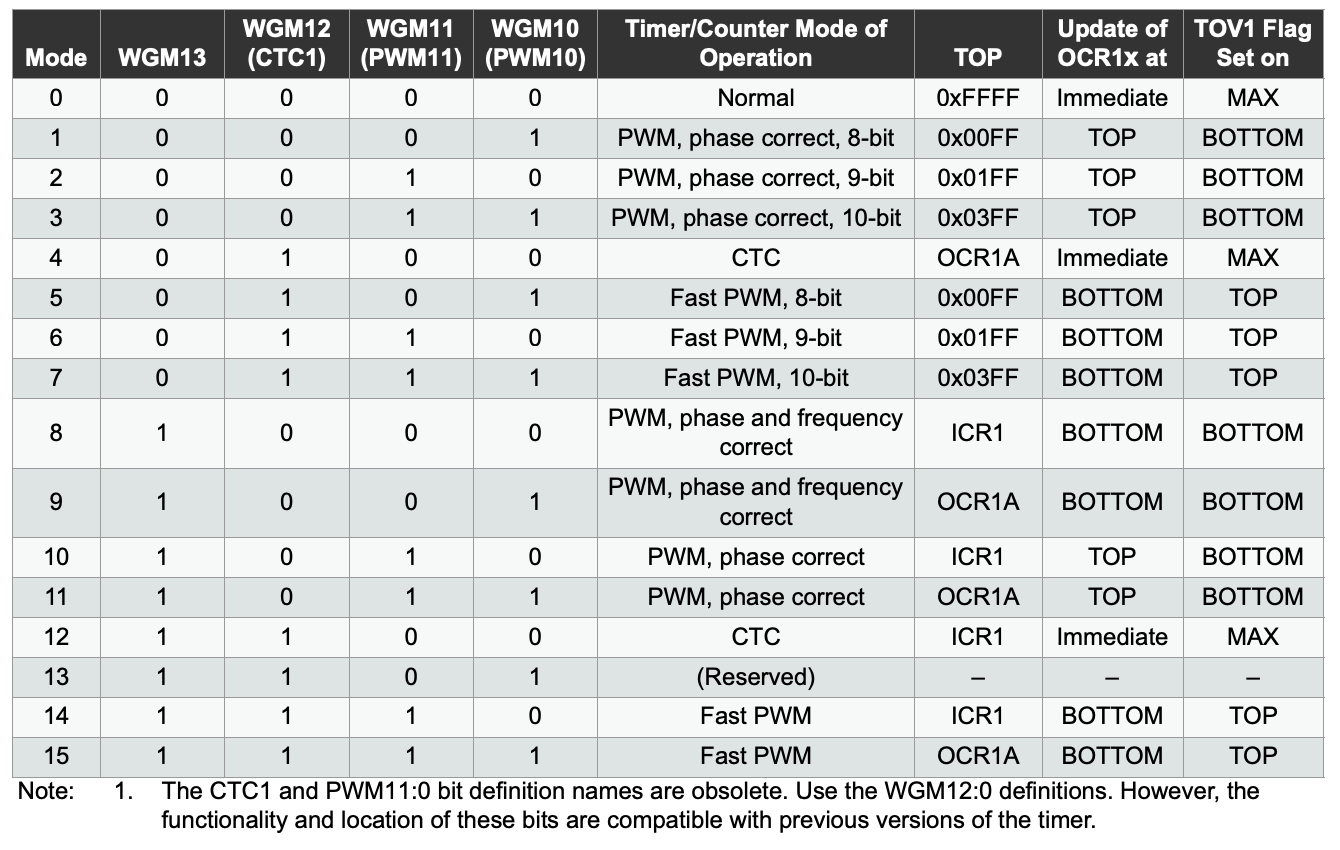
\includegraphics[width=15cm]{WGM-Timer1}
    \caption{Waveform Generation Mode Bit Description for Timer1. \tiny Copied from ATmega382P Data Sheet, Table~15-5 \label{fig:Timer1WGM}}
\end{figure}

\begin{figure}
    \centering
    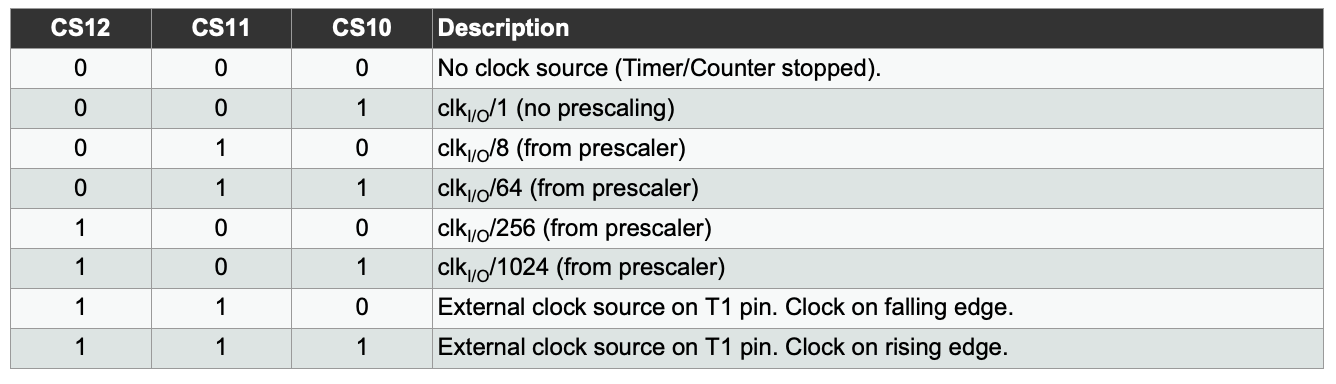
\includegraphics[width=15cm]{CS-Timer1}
    \caption{Clock Select Bit Description for Timer1. \tiny Copied from ATmega382P Data Sheet, Table~15-6 \label{fig:Timer1CS}}
\end{figure}

\begin{figure}
    \centering
    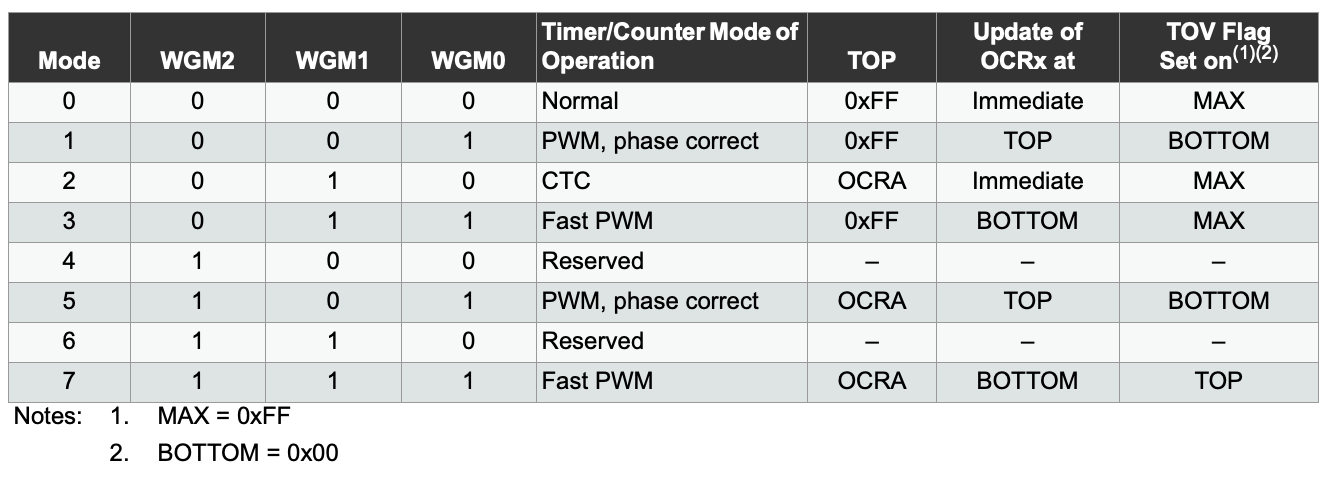
\includegraphics[width=15cm]{WGM-Timer2}
    \caption{Waveform Generation Mode Bit Description for Timer2. \texttt{WGM22}, \texttt{WGM21}, and \texttt{WGM20} are incorrectly shown here as \texttt{WGM2}, \texttt{WGM1}, and \texttt{WGM0}. \texttt{OCR2A} is incorrectly shown here as \texttt{OCRA}. \tiny Copied from ATmega382P Data Sheet, Table~17-8 \label{fig:Timer2WGM}}
\end{figure}

\begin{figure}
    \centering
    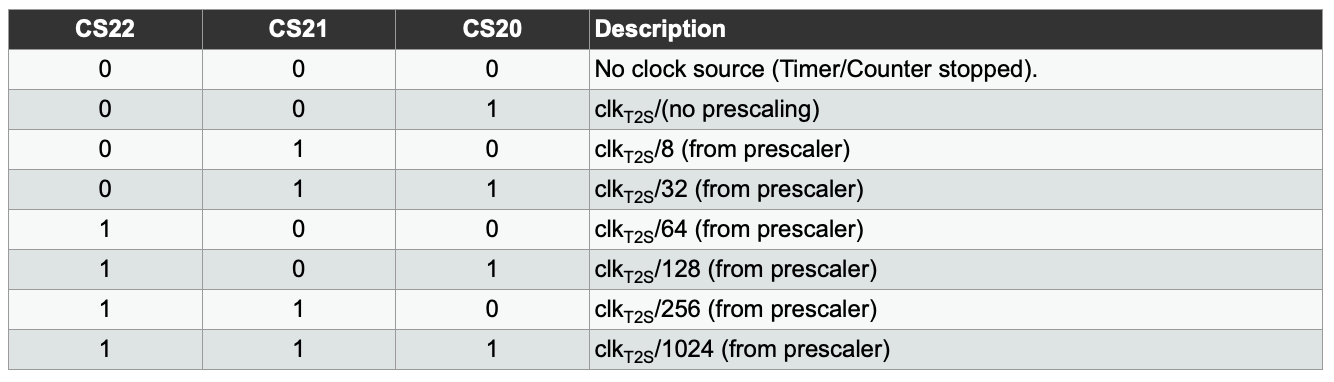
\includegraphics[width=15cm]{CS-Timer2}
    \caption{Clock Select Bit Description for Timer2. \tiny Copied from ATmega382P Data Sheet, Table~17-9 \label{fig:Timer2CS}}
\end{figure}

\begin{table}
    \centering \small
    \begin{tabular}{|r||c|c|c|c||}
        \hline
        Bits                & \textbf{31..24}   & \textbf{23..16}   & \textbf{15..8}    & \textbf{7..0}     \\ \cline{2-5}
        \textbf{control}    & \textit{reserved} & \texttt{TCCR1C}   & \texttt{TCCR1B}   & \texttt{TCCR1A}   \\
        \textbf{counter}    & \multicolumn{2}{c|}{}                 & \multicolumn{2}{c||}{\texttt{TCNT1}}  \\
        \textbf{capture}    & \multicolumn{2}{c|}{}                 & \multicolumn{2}{c||}{\texttt{ICR1}}   \\
        \textbf{compareA}   & \multicolumn{2}{c|}{}                 & \multicolumn{2}{c||}{\texttt{OCR1A}}  \\
        \textbf{compareB}   & \multicolumn{2}{c|}{}                 & \multicolumn{2}{c||}{\texttt{OCR1B}}  \\ \hline
    \end{tabular}
    \caption{Relationship of \lstinline{timer_registers_16bit} fields to Timer1's registers. \tiny Adapted from ATmega382P Data Sheet, §15.11. \label{table:Timer1Registers}}
\end{table}

\begin{table}
    \centering \small
    \begin{tabular}{|r||c|c|c|c|c|c|c|c||}
        \hline
        Bit             & \textbf{7}        & \textbf{6}        & \textbf{5}        & \textbf{4}        & \textbf{3}        & \textbf{2}    & \textbf{1}        & \textbf{0}        \\ \cline{2-9}
        \textbf{TCCR1C} & \texttt{FOC1A}    & \texttt{FOC1B}    & -                 & -                 & -                 & -             & -                 & -                 \\
        \textbf{TCCR1B} & \texttt{ICNC1}    & \texttt{ICES1}    & -                 & \texttt{WGM13}    & \texttt{WGM12}    & \texttt{CS12} & \texttt{CS11}     & \texttt{CS10}     \\
        \textbf{TCCR1A} & \texttt{COM1A1}   & \texttt{COM1A0}   & \texttt{COM1BA1}  & \texttt{COM1B0}   & -                 & -             & \texttt{WGM11}    & \texttt{WGM10}    \\ \hline
    \end{tabular}
    \caption{Timer1's control registers. \tiny Adapted from ATmega382P Data Sheet, §15.11. \label{table:Timer1Control}}
\end{table}

\begin{table}
    \centering \small
    \begin{tabular}{|r||c|c||}
        \hline
        Bits                & \textbf{15..8}    & \textbf{7..0}     \\ \cline{2-3}
        \textbf{control}    & \texttt{TCCR2B}   & \texttt{TCCR2A}   \\
        \textbf{counter}    &                   & \texttt{TCNT2}    \\
        \textbf{compareA}   &                   & \texttt{OCR2A}    \\
        \textbf{compareB}   &                   & \texttt{OCR2B}    \\ \hline
    \end{tabular}
    \caption{Relationship of \lstinline{timer_registers_8bit} fields to Timer2's registers. \tiny Adapted from ATmega382P Data Sheet, §17.11. \label{table:Timer2Registers}}
\end{table}

\begin{table}
    \centering \small
    \begin{tabular}{|r||c|c|c|c|c|c|c|c||}
        \hline
        Bit             & \textbf{7}        & \textbf{6}        & \textbf{5}        & \textbf{4}        & \textbf{3}        & \textbf{2}    & \textbf{1}        & \textbf{0}        \\ \cline{2-9}
        \textbf{TCCR2B} & \texttt{FOC2A}    & \texttt{FOC2B}    & -                 & -                 & \texttt{WGM22}    & \texttt{CS22} & \texttt{CS21}     & \texttt{CS20}     \\
        \textbf{TCCR2A} & \texttt{COM2A1}   & \texttt{COM2A0}   & \texttt{COM2BA1}  & \texttt{COM2B0}   & -                 & -             & \texttt{WGM21}    & \texttt{WGM20}    \\ \hline
    \end{tabular}
    \caption{Timer2's control registers. \tiny Adapted from ATmega382P Data Sheet, §17.11. \label{table:Timer2Control}}
\end{table}

Next assign your computed $comparison\_value$ the struct's \lstinline{compareA}
field, or to OCR1A (Timer1) or OCR2A (Timer2), as appropriate.

Finally, enable the comparison-based timer interrupt. If you are using
memory-mapped I/O:
\begin{itemize}
\item Create a pointer to a \lstinline{volatile uint8_t} and assign to it the
    address \lstinline{IObase + 0x4E}.
\item Treat the pointer as an array, and use the timer number (1 or 2) for the
    index when making an assignment.
\end{itemize}
If you are using AVR-libc macros:
\begin{itemize}
\item Make an assignment to \texttt{TIMSK1} for Timer1, or to \texttt{TIMSK2}
    for Timer2.
\end{itemize}

You want to place a 1 in the \texttt{OCIEnA} bit (where $n$ is the timer
number); use Figure~\ref{fig:TimerInterruptRegisters} to determine the
appropriate bit to set.

\begin{figure}
    \centering
    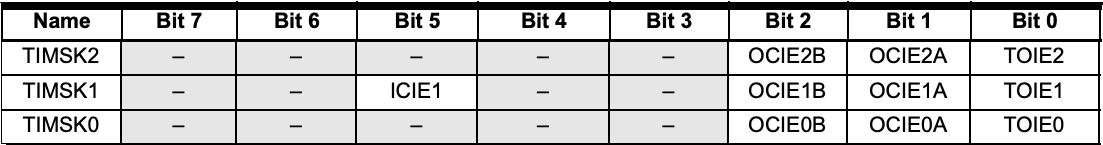
\includegraphics[width=15cm]{TimerInterruptRegisters}
    \caption{Timer interrupt registers. \tiny Cropped from ATmega382P Data Sheet, §30 \label{fig:TimerInterruptRegisters}}
\end{figure}


\subsection{Interrupt Service Routine}

Because the Arduino core does not provide a more convenient way to create an
interrupt service routine (ISR) for timer interrupts, you will use AVR-libc's
\function{ISR}\footnote{\url{https://www.nongnu.org/avr-libc/user-manual/group__avr__interrupts.html}}
macro.

In \textit{CalculatorLab.ino}, outside of any other function, write this code that looks like a function:

\begin{lstlisting}
ISR(vector) {
    ...
}
\end{lstlisting}

where $vector$ is \lstinline{TIMER1_COMPA_vect} for Timer1 or
\lstinline{TIMER2_COMPA_vect} for Timer2. Replace ``\dots'' with the code that
should execute whenever the timer interrupt occurs. You want to keep your ISR
short, no more than a few lines of code. If anything more elaborate needs to
happen, code in your \function{loop()} function (or a function called by
\function{loop()}) can do that based on changes made from within your ISR.

Initially, you may want to simply place a \function{println} statement in your
ISR code to verify that you have the timing correct. Once you are satisfied
that you have done so, remove the \function{println} statement and add the code
you need for your logic.

\textbf{NOTE} Any global variables used by your ISR should be declared as \lstinline{volatile}.

\textbf{NOTE} If you ever need to ``reset'' a timer's count back to 0, you can
simply write 0 to the structs \lstinline{counter} field or to
\texttt{TCNT1}/\texttt{TCNT2}.

\section{Yada} \label{sec:yada}

\dots

\subsubsection{Blah}


\section*{Turn-in and Grading}

When you have completed this assignment, upload \textit{InterruptLab.ino} to
\filesubmission.

This assignment is worth 30 or 35 or 40 points. \\

Rubric:
% \begin{description}
% \rubricitem{8}{Simple input/output functions correctly. (3 points for switches; 3 points for pushbuttons; 2 points for LED)}
% \rubricitem{10}{Matrix keypad functions correctly.}
% \rubricitem{8}{7-Segment Display Module functions correctly.}
% \rubricitem{1}{System is in demonstration mode only when left switch is in left position and builder mode when the left switch is in the right position.}
% \rubricitem{1}{External LED illuminates when key is pressed and deluminates 500ms later if in demonstration mode. (This behavior is unspecified when in building mode.)}
% \rubricitem{2}{When in demonstration  mode, the numeral corresponding to the key pressed is displayed in the least-significant digit on the Display Module, in accordance with requirements~\ref{spec:decimalExplained}, \ref{spec:hexadecimalExplained}, and \ref{spec:demonstrationKeyPress}. (1 point for decimal number base; 1 point for hexadecimal number base)}
% \rubricitem{1}{When in demonstration mode, the right pushbutton clears the display.}
% \rubricitem{2}{Builds a value consistent with requirements~\ref{spec:decimalExplained} and \ref{spec:BuildingValue} when in building mode and using the decimal number base. (\textonehalf\ point for each of: printing correct positive values, printing correct negative values, displaying correct positive values, displaying correct negative values)}
% \rubricitem{2}{Builds a value consistent with requirements~\ref{spec:hexadecimalExplained} and \ref{spec:BuildingValue} when in building mode and using the hexadecimal number base. (\textonehalf\ point for each of: printing correct positive values, printing correct negative values, displaying correct positive values, displaying correct negative values)}
% \rubricitem{1}{Negates value in the decimal number base when left pushbutton is pressed while in building mode. (\textonehalf\ point for each of: printing and displaying correct positive values, printing and displaying correct negative values)}
% \rubricitem{1}{Negates value in the hexadecimal number base when left pushbutton is pressed while in building mode. (\textonehalf\ point for each of: storing and displaying correct positive values, storing and displaying correct negative values)}
% \rubricitem{2}{Detects and displays correct message when the number being built is too big. (\textonequarter\ point for detecting too-big numbers for each of: positive decimal numbers, negative decimal numbers, positive hexadecimal numbers, negative hexadecimal numbers; \textonequarter\ point for no false detections among each of: decimal numbers, hexadecimal numbers; \textonehalf\ point for printing the correct message)}
% \rubricitem{1}{When in building mode the right pushbutton clears all digits on the Display Module except the least-significant digit, which displays {\dviiseg 0}.}
% \bonusitem{2}{Get assignment checked-off by TA or professor during office hours before it is due. (You cannot get both bonuses.)}
% \bonusitem{1}{Get assignment checked-off by TA at \textit{start} of your scheduled lab immediately after it is due. (Your code must be uploaded to \filesubmission\ \textit{before} it is due. You cannot get both bonuses.)}
% \item[Penalties]
% \penaltyitem{8}{Simple input/output configuration and test function relies on code that violates the constraints in Section~\ref{sec:Constraints}.}
% \penaltyitem{10}{Obtaining values from matrix keypad relies on code that violates the constraints in Section~\ref{sec:Constraints}.}
% \penaltyitem{8}{Sending values to the 7-segment display module relies on code that violates the constraints in Section~\ref{sec:Constraints}.}
% \penaltyitem{5}{Code associated with demonstration mode (other than that covered in the first three penalty items) relies on code that violates the constraints in Section~\ref{sec:Constraints}.}
% \penaltyitem{9}{Code associated with conversion mode (other than that covered in the first three penalty items) relies on code that violates the constraints in Section~\ref{sec:Constraints}.}
% \spaghetticodepenalties{1}
% \end{description}

\section*{Epilogue}

% Herb looks over your work. ``Hmm, yes. I think this is coming along nicely.
% Let's run a few more tests.''
%
% Archie storms into the room. ``We have \textit{got} to do something about
% security! How's that doodad coming along? Because there's now a
%  half-man/half-fly in the labs going on-and-on about Chaos Theory and how if we
%  just give him a MacBook and a spaceship then he'll be able to get the Lord of
%  Thunder to travel across the 8th Dimension. Is that thing just about ready?''
%
% Herb shakes his head, ``No, not quite yet. It should be ready in about a week.''

\textit{To be continued...}

\newpage

\section*{Appendix: Lab Checkoff}

You are not required to have your assignment checked-off by a TA or the
professor. If you do not do so, then we will perform a functional check
ourselves. In the interest of making grading go faster, we are offering a small
bonus to get your assignment checked-off at the start of your scheduled lab
time immediately after it is due. Because checking off all students during lab
would take up most of the lab time, we are offering a slightly larger bonus if
you complete your assignment early and get it checked-off by a TA or the
professor during office hours.

% \begin{description}
% \item [] (\phantom{xxx}) Establish that the code you are demonstrating is the code
%     you submitted to to \filesubmission.
%     \begin{itemize}
%     \item If you are getting checked-off during lab time, show the TA that the
%         file was submitted before it was due.
%     \item Download the file into your PollingLab directory. If necessary,
%         rename it to \textit{PollingLab.ino}.
%     \end{itemize}
% \item [] (\phantom{xxx}) Upload \textit{PollingLab.ino} to your \nano.
% \end{description}
% \textbf{If you completed demonstration mode, jump ahead to
% \textit{Demonstration Mode}.} Successfully completing demonstration
% \textit{prima facie} shows that the I/O functions correctly.
%
% \textbf{If you did not complete demonstration mode:}
% \renewcommand{\labelenumi}{\Alph{enumi}.}
% \begin{enumerate}
% \item (\phantom{xxx}) Using \function{testSimpleIO()}, show on the Serial
%     Monitor that the left and right button presses are detected. \\
%     \textit{+1\textonehalf\ pushbutton presses detected} \\
%     \textit{+1\textonehalf\ left and right pushbuttons are distinguished from
%     each other}
% \item (\phantom{xxx}) Using \function{testSimpleIO()}, show on the Serial
%     Monitor that the left and right switches' position changes are detected. \\
%     \textit{+1\textonehalf\ switch positions detected} \\
%     \textit{+1\textonehalf\ left and right switches are distinguished from
%     each other}
% \item (\phantom{xxx}) Show that the external LED illuminates when it is
%     supposed to (in a bright room, you may need to shade the LED with your
%     hand). You can do this either by moving both switches to the right position
%     (using the code in \function{testSimpleIO()}) or by showing the LED
%     illuminate when you press a key on the matrix keypad (if you started
%     working on demonstration mode). \\
%     \textit{+2 LED works}
% \item (\phantom{xxx}) Show on the Serial Monitor that key presses on the matrix
%     keypad are correctly decoded. \\
%     \textit{+10 keypad works}
% \item (\phantom{xxx}) Show on the display module that values decoded from the
%     matrix keypad are displayed as the correct characters. \\
%     \textit{+8 display module works}
% \end{enumerate}
% \renewcommand{\labelenumi}{\arabic{enumi}.}
% \begin{enumerate}
% \item [] \textbf{\textit{Demonstration Mode}}
% \item (\phantom{xxx}) Place both switches in the left position. The display
%     module is initially blank.
% \item(\phantom{xxx}) Press a number key on the matrix keypad. The corresponding
%     character appears on the display module, and the external LED illuminates
%     for approximately one-half of a second. \\
%     \textit{+1 LED illumination} \\
%     \textit{+2 LED works}
% \item (\phantom{xxx}) Press a different number key on the matrix keypad.
%     The corresponding character appears on the display module, and the external
%     LED illuminates for approximately one-half of a second. \\
%     \textit{+\textonehalf\ decimal numeral} \\
%     \textit{+10 keypad works} \\
%     \textit{+8 display module works}
% \item (\phantom{xxx}) Press a letter key on the matrix keypad. The display
%     module is unchanged. \\
%     \textit{+\textonehalf\ letter rejected in decimal number base}
% \item (\phantom{xxx}) Place the right switch in the right position. The display
%     is unchanged.
% \item (\phantom{xxx}) Press a letter key on the matrix keypad. The
%     corresponding character appears on the display module, and the external LED
%     illuminates for approximately one-half of a second. \\
%     \textit{+1 hexadecimal numeral} \\
%     \textit{+1\textonehalf\ switch positions detected}
% \item (\phantom{xxx}) Press the right pushbutton. The display module blanks. \\
%     \textit{+1 clear display} \\
%     \textit{+1\textonehalf\ pushbutton presses detected}
% \item (\phantom{xxx}) Press a key on the matrix keypad. The corresponding
%     character appears on the display module, and the external LED illuminates
%     for approximately one-half of a second. \\
%     \textit{establishes that demonstration mode continues to work; if not then
%     deduct half of the decimal/hexadecimal numeral points (if any)}
% \item (\phantom{xxx}) Press the same key on the matrix keypad. The display
%     module is unchanged (still displays the corresponding character), but the
%     external LED still illuminates for approximately one-half of a second. \\
%     \textit{establishes that the same key can be pressed twice with
%     well-defined behavior; if the display changes then deduct half of the
%     decimal/hexadecimal numeral points (if any); if the LED does not illuminate
%     then deduct half of the ``LED illumination'' point (if any) but not the
%     ``LED works'' points}
% \item (\phantom{xxx}) Press the left pushbutton. Nothing happens. \\
%     \textit{+1\textonehalf\ left and right pushbuttons are distinguished from
%     each other}
% \item[] \textbf{\textit{Demonstration Mode and Building Mode are Different}}
% \item (\phantom{xxx}) Place the left switch in the right position. The display
%     remains unchanged.
% \item (\phantom{xxx}) Press the right pushbutton. The display shows \\
%     {\dviiseg\phantom{0000000}0}\hspace{1cm}(additional leading 0s are allowed)
%     \\ and the Serial Monitor shows \\
%     {\dviiseg\phantom{00000000}}\hspace{1cm}\texttt{0} \\
%     \textit{+1 left switch selects mode} \\
%     \textit{+1\textonehalf\ left and right switches are distinguished from
%     each other}
% \item[] \textbf{\textit{Building Mode}}
% \item (\phantom{xxx}) Place the right switch in the left position. The display
%     remains unchanged.
% \item (\phantom{xxx}) Press 2, then 3. \\
%     {\dviiseg \phantom{0000000}2}\hspace{1cm}\texttt{2} \\
%     {\dviiseg \phantom{000000}23}\hspace{1cm}\texttt{23}
% \item (\phantom{xxx}) Press B. The display is unchanged. \\
%     \textit{printing (+\textonehalf) \& displaying (+\textonehalf) positive decimal numbers}
% \item (\phantom{xxx}) Press the left pushbutton, then 1. \\
%     {\dviiseg \phantom{00000}-23}\hspace{1cm}\texttt{-23}\hspace{1cm}
%     \textit{+\textonehalf\ negates decimal positive values} \\
%     {\dviiseg \phantom{0000}-231}\hspace{1cm}\texttt{-231}\hspace{1cm}
%     \textit{printing (+\textonehalf) \& displaying (+\textonehalf) negative decimal numbers}
% \item (\phantom{xxx}) Press the left pushbutton, then 4. \\
%     {\dviiseg \phantom{00000}231}\hspace{1cm}\texttt{231}\hspace{1cm}
%     \textit{+\textonehalf\ negates decimal negative values} \\
%     {\dviiseg \phantom{0000}2314}\hspace{1cm}\texttt{2314}\hspace{1cm}
%     \textit{establishes that building mode continues to work}
% \item (\phantom{xxx}) Press D. The display is unchanged. \\
%     \textit{establishes that building mode continues to work; if building mode
%     does not work after negation, deduct half of the printing/displaying
%     decimal points (if any)}
% \item (\phantom{xxx}) Press the right pushbutton, and place the right switch in
%     the right position. \\
%     {\dviiseg\phantom{0000000}0}\hspace{1cm}\texttt{0}\hspace{1cm}
%     \textit{+1 display resets to 0}
% \item(\phantom{xxx}) Press \#, then 7. \\
%     {\dviiseg \phantom{0000000}E}\hspace{1cm}\texttt{E} \\
%     {\dviiseg \phantom{000000}E7}\hspace{1cm}\texttt{E7}\hspace{1cm}
%     \textit{printing (+\textonehalf) \& displaying (+\textonehalf) positive hex
%     numbers}
% \item (\phantom{xxx}) Press the left pushbutton. \\
%     {\dviiseg FFFFFF19}\hspace{1cm}\texttt{FFFFFF19}\hspace{1cm}
%     \textit{+\textonehalf\ negates hex positive values}
% \item(\phantom{xxx}) Press 0, then A. \\
%     {\dviiseg FFFFF190}\hspace{1cm}\texttt{FFFFF190} \\
%     {\dviiseg FFFF190A}\hspace{1cm}\texttt{FFFF190A}\hspace{1cm}
%     \textit{printing (+\textonehalf) \& displaying (+\textonehalf) negative hex
%     numbers}
% \item(\phantom{xxx}) Press the left pushbutton, then *. \\
%     {\dviiseg \phantom{0000}E6F6}\hspace{1cm}\texttt{E6F6}\hspace{1cm}
%     \textit{+\textonehalf\ negates hex negative values} \\
%     {\dviiseg \phantom{000}E6F6F}\hspace{1cm}\texttt{E6F6F}\hspace{1cm}
%     \textit{establishes that building mode continues to work}
% \item(\phantom{xxx}) Press B, then C, then D, then 0. \\
%     {\dviiseg \phantom{00}E6F6FB}\hspace{1cm}\texttt{E6F6FB} \\
%     {\dviiseg \phantom{0}E6F6FBC}\hspace{1cm}\texttt{E6F6FBC} \\
%     {\dviiseg           E6F6FBCD}\hspace{1cm}\texttt{E6F6FBCD}\hspace{1cm}
%     \textit{no false detection - hex \#1} \\
%     {\dviiseg \phantom{0}too big}\hspace{1cm}\texttt{too big}\hspace{1cm}
%     \textit{too big - negative hex \#1}
% \item (\phantom{xxx}) Press the right pushbutton; then press 1, then 2, then 3, then A, then B, then 6, then 5, then 4, then 7. \\
%     {\dviiseg \phantom{0000000}0}\hspace{1cm}\texttt{0} \\
%     {\dviiseg \phantom{0000000}1}\hspace{1cm}\texttt{1} \\
%     {\dviiseg \phantom{000000}12}\hspace{1cm}\texttt{12} \\
%     {\dviiseg \phantom{00000}123}\hspace{1cm}\texttt{123} \\
%     {\dviiseg \phantom{0000}123A}\hspace{1cm}\texttt{123A} \\
%     {\dviiseg \phantom{000}123AB}\hspace{1cm}\texttt{123AB} \\
%     {\dviiseg \phantom{00}123AB6}\hspace{1cm}\texttt{123AB6} \\
%     {\dviiseg \phantom{0}123AB65}\hspace{1cm}\texttt{123AB65} \\
%     {\dviiseg           123AB654}\hspace{1cm}\texttt{123AB654}\hspace{1cm}
%     \textit{no false detection - hex \#2} \\
%     {\dviiseg \phantom{0}too big}\hspace{1cm}\texttt{too big}\hspace{1cm}
%     \textit{+\textonequarter\ too big - positive hex}
% \item (\phantom{xxx}) Press the right pushbutton; then push *, then 2, then 3, then A, then B, then 6, then 5, then 4, then 7. \\
%     {\dviiseg \phantom{0000000}0}\hspace{1cm}\texttt{0} \\
%     {\dviiseg \phantom{0000000}F}\hspace{1cm}\texttt{F} \\
%     {\dviiseg \phantom{000000}F2}\hspace{1cm}\texttt{F2} \\
%     {\dviiseg \phantom{00000}F23}\hspace{1cm}\texttt{F23} \\
%     {\dviiseg \phantom{0000}F23A}\hspace{1cm}\texttt{F23A} \\
%     {\dviiseg \phantom{000}F23AB}\hspace{1cm}\texttt{F23AB} \\
%     {\dviiseg \phantom{00}F23AB6}\hspace{1cm}\texttt{F23AB6} \\
%     {\dviiseg \phantom{0}F23AB65}\hspace{1cm}\texttt{F23AB65} \\
%     {\dviiseg           F23AB654}\hspace{1cm}\texttt{F23AB654}\hspace{1cm}
%     \textit{no false detection - hex \#3} \\
%     {\dviiseg \phantom{0}too big}\hspace{1cm}\texttt{too big}\hspace{1cm}
%     \textit{too big - negative hex \#2}
% \item (\phantom{xxx}) Press the right pushbutton; then push *, then 9, then 3, then A, then B, then 6, then 5, then 4, then 7, then 8. \\
%     {\dviiseg \phantom{0000000}0}\hspace{1cm}\texttt{0} \\
%     {\dviiseg \phantom{0000000}F}\hspace{1cm}\texttt{F} \\
%     {\dviiseg \phantom{000000}F9}\hspace{1cm}\texttt{F9} \\
%     {\dviiseg \phantom{00000}F93}\hspace{1cm}\texttt{F93} \\
%     {\dviiseg \phantom{0000}F93A}\hspace{1cm}\texttt{F93A} \\
%     {\dviiseg \phantom{000}F93AB}\hspace{1cm}\texttt{F93AB} \\
%     {\dviiseg \phantom{00}F93AB6}\hspace{1cm}\texttt{F93AB6} \\
%     {\dviiseg \phantom{0}F93AB65}\hspace{1cm}\texttt{F93AB65} \\
%     {\dviiseg           F93AB654}\hspace{1cm}\texttt{F93AB654} \\
%     {\dviiseg           93AB6547}\hspace{1cm}\texttt{93AB6547}\hspace{1cm}
%     \textit{no false detection - hex \#4} \\
%     {\dviiseg \phantom{0}too big}\hspace{1cm}\texttt{too big}\hspace{1cm}
%     \textit{too big - negative hex \#3} \\
%     \textit{+\textonequarter\ for all three ``too bit - negative hex''} \\
%     \textit{+\textonequarter\ for all four ``no false detection - hex''}
% \item (\phantom{xxx}) Press the right pushbutton, and place the right switch in
%     the left position. \\
%     {\dviiseg \phantom{0000000}0}\hspace{1cm}\texttt{0}
% \item (\phantom{xxx}) Press 5, then 6, then 7, then 8, then 9, then 0, then 1, then 2, then 3. \\
%     {\dviiseg \phantom{0000000}5}\hspace{1cm}\texttt{5} \\
%     {\dviiseg \phantom{000000}56}\hspace{1cm}\texttt{56} \\
%     {\dviiseg \phantom{00000}567}\hspace{1cm}\texttt{567} \\
%     {\dviiseg \phantom{0000}5678}\hspace{1cm}\texttt{5678} \\
%     {\dviiseg \phantom{000}56789}\hspace{1cm}\texttt{56789} \\
%     {\dviiseg \phantom{00}567890}\hspace{1cm}\texttt{567890} \\
%     {\dviiseg \phantom{0}5678901}\hspace{1cm}\texttt{5678901} \\
%     {\dviiseg           56789012}\hspace{1cm}\texttt{56789012}\hspace{1cm}
%     \textit{no false detection - decimal \#1} \\
%     {\dviiseg \phantom{0}too big}\hspace{1cm}\texttt{too big}\hspace{1cm}
%     \textit{+\textonequarter\ too big - positive decimal}
% \item (\phantom{xxx}) Press the right pushbutton; then press 3, then the left pushbutton, then 4, then 5, then 6, then 7, then 8, then 9, then 0. \\
%     {\dviiseg \phantom{0000000}0}\hspace{1cm}\texttt{0} \\
%     {\dviiseg \phantom{0000000}3}\hspace{1cm}\texttt{3} \\
%     {\dviiseg \phantom{000000}-3}\hspace{1cm}\texttt{-3} \\
%     {\dviiseg \phantom{00000}-34}\hspace{1cm}\texttt{-34} \\
%     {\dviiseg \phantom{0000}-345}\hspace{1cm}\texttt{-345} \\
%     {\dviiseg \phantom{000}-3456}\hspace{1cm}\texttt{-3456} \\
%     {\dviiseg \phantom{00}-34567}\hspace{1cm}\texttt{-34567} \\
%     {\dviiseg \phantom{0}-345678}\hspace{1cm}\texttt{-345678} \\
%     {\dviiseg           -3456789}\hspace{1cm}\texttt{-3456789}\hspace{1cm}
%     \textit{no false detection - decimal \#2} \\
%     {\dviiseg \phantom{0}too big}\hspace{1cm}\texttt{too big}\hspace{1cm}
%     \textit{+\textonequarter\ too big - negative decimal} \\
%     \textit{+\textonequarter\ for both ``no false detection - decimal''} \\
%     \textit{+\textonehalf\ if all ``too big'' displayed the correct message;
%     +\textonequarter\ if all but one ``too big'' displayed the correct message}
% \end{enumerate}
%
% This concludes the demonstration of your system's functionality. The TAs will
% later examine your code for violations of the assignment's constraints. If your
% code looks like it is tailored for this checklist, the TAs may re-grade using a
% different checklist\texttt{.}
\end{document}
